\section{Esamų sistemų pertvarkymas}
Apibrėžus šablonus paketų skirstymui galima pradėti vertinti jų įtaką sistemai, juos pritaikant esamoms sistemoms.
Šio skyriaus tikslas - pasirinkti ir išnagrinėti kelias sistemas, pasitelkus paketų kokybės matus, bei bendrą sistemos struktūros analizę,
taip identifikuojant programiniam kodui būdingas problemas, rastas problemas išspręsti pritaikant aprašytus šablonus.
Atlikus pertvarkymus sistemose, dar kartą paskaičiuoti paketų kokybės matus,
taip gaunant įrodymus, ar gauti šablonai yra efektyvūs ir iš tiesų sprendžia
jiems priskirtas problemas.


\subsection{Sistemų pasirinkimas}
Sistemų pertvarkymui pasirinktos atviro kodo sistemos, kurių kodas yra viešai prietinamas \textit{github} platformoje.
Pasirinktos sistemos yra vidutinio dydžio, todėl nėra labai sudėtinga jas suprasti ir pertvarkyti, bet taip pat jos nėra
tokios paprastos, kad neturėtų sistemos dizaino problemų.
Pasirinktos sistemos yra skirtingo tipo projektai, taip užtikrinant didesnę problemų ivairovę ir objektyvesnius įvertinimus.
Per visą pasirinktų sistemų imtį yra sutinkamos visos aprašytos problemos, taip įvertinant visus aprašytus šablonus.

\subsection{\textit{Leaf} sistema}
\textbf{Leaf\footnote{\url{https://github.com/Meituan-Dianping/Leaf/tree/master}}} sistema, per \textit{http}
protokolą teikianti aplikacijų programavimo sąsają unikalaus identifikatoriaus generavimui.
Ši sistema užtikrina identifikatoriaus unikalų pasiskirstymą tarp skirtingų paskirstytų sistemų \angl{distributed systems},
servisais orientuotoje \angl{service-oriented} architektūroje.
Tai techninės programinės įrangos tipas, kuris naudojamas kitų taikomosios programinės įrangos sistemų.
Sistema Leaf susideda iš dviejų modulių \textit{server} ir \textit{core}, šiame darbe dėmesys bus skirtas tik \textit{core} moduliui,
kadangi \textit{server} modulis yra labai mažas
ir paketų struktūra jame neatlieka esminio vaidmens.
Prieš visus pakeitimus \textit{Leaf} sistemos, \textit{core} modulio paketų struktūra atrodo taip:
\begin{figure}[H]
    \centering
    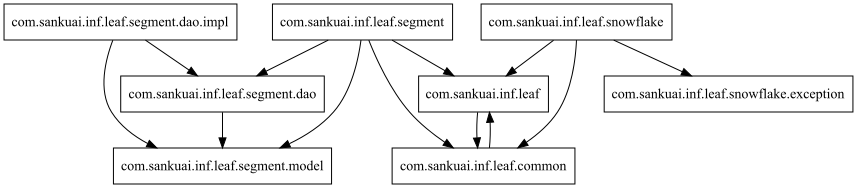
\includegraphics[scale=0.5]{img/leaf_packages_orig}
    \caption{\textit{Leaf} sistemos \textit{core} modulio struktūra}
    \label{img:leaf_packages_orig}
\end{figure}

\dirtree{%
.1 {/}.
.2 {common}.
.2 {segment}.
.3 {dao}.
.4 {impl}.
.3 {model}.
.2 {snowflake}.
.3 {exception}.
}

\begin{center}
    \begin{tabular}{|c|c|c|c|c|c|c|}
        \hline
        Paketo vardas & \textit{N} & \textit{A} & \textit{E} & \textit{S} & \textit{A} & \textit{D} \\ [0.5ex]
        \hline\hline
        leaf.segment.dao.impl & 1 & 0 & 2 & 1.0 & 0.0 & 0.0 \\
        \hline
        leaf.segment & 1 & 0 & 4 & 1.0 & 0.0 & 0.0 \\
        \hline
        leaf.snowflake.exception & 3 & 1 & 0 & 0.0 & 0.0 & 1.0 \\
        \hline
        leaf.segment.model & 3 & 3 & 0 & 0.0 & 0.0 & 1.0 \\
        \hline
        leaf.segment.dao & 2 & 2 & 1 & 0.333 & 1.0 & 0.333 \\
        \hline
        leaf & 1 & 3 & 1 & 0.25 & 1.0 & 0.25 \\
        \hline
        leaf.common & 6 & 3 & 1 & 0.25 & 0.0 & 0.75 \\
        \hline
        leaf.snowflake & 2 & 0 & 3 & 1.0 & 0.0 & 0.0 \\
        \hline
    \end{tabular}
    \begin{tabular}{|c|c|c|c|c|c|}
        \hline
        $\bar{N}$ & $\bar{A}$ & $\bar{E}$ & $\bar{S}$ & $\bar{A}$ & $\bar{D}$ \\ [0.5ex]
        \hline\hline
        2 & 2 & 2 & 0.479 & 0.25 & 0.417 \\
        \hline
    \end{tabular}
\end{center}
